
The goal of this chapter is ...

\section{Time on air}

\subsection{Regulations}

\subsection{Lab tests}

\begin{figure}[ht]
    \centering
    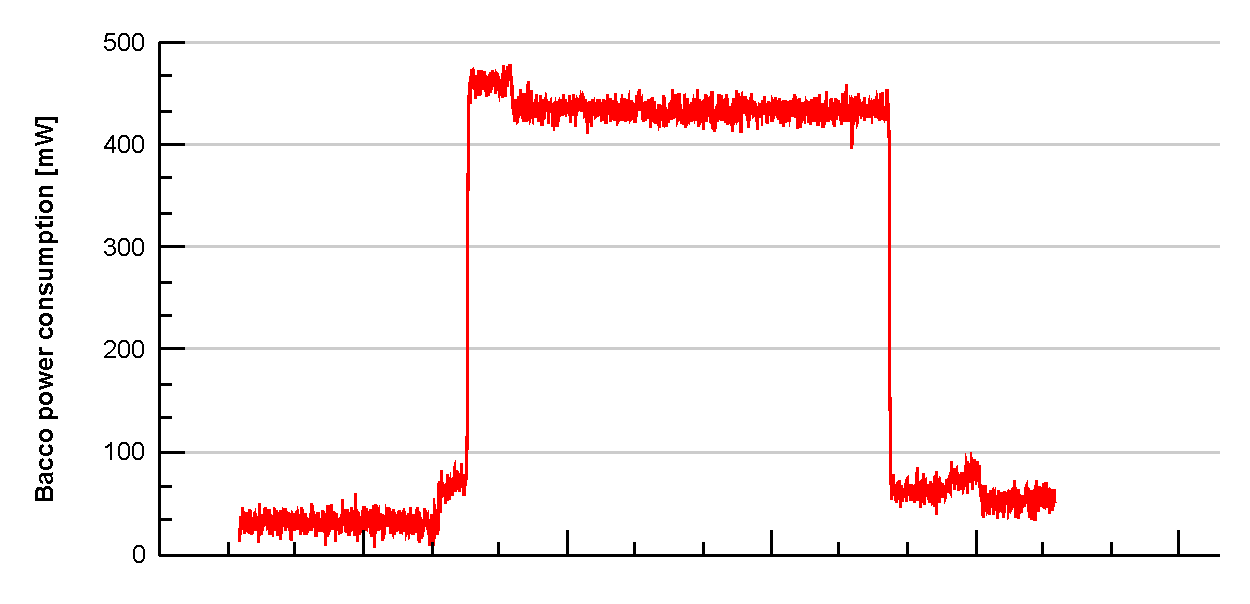
\includegraphics[width=1.0\textwidth]{images/bacco_SF7_14dbm_125khz_power.pdf}
    \caption{Power draw during transmission of a Bacco packet with payload size of 15 bytes, using SF7, 14dBm, 125kHz bandwidth}
    \label{bacco SF7}
\end{figure}
delta time is 51.6ms and total energy is 21.3mJ

\begin{figure}[ht]
    \centering
    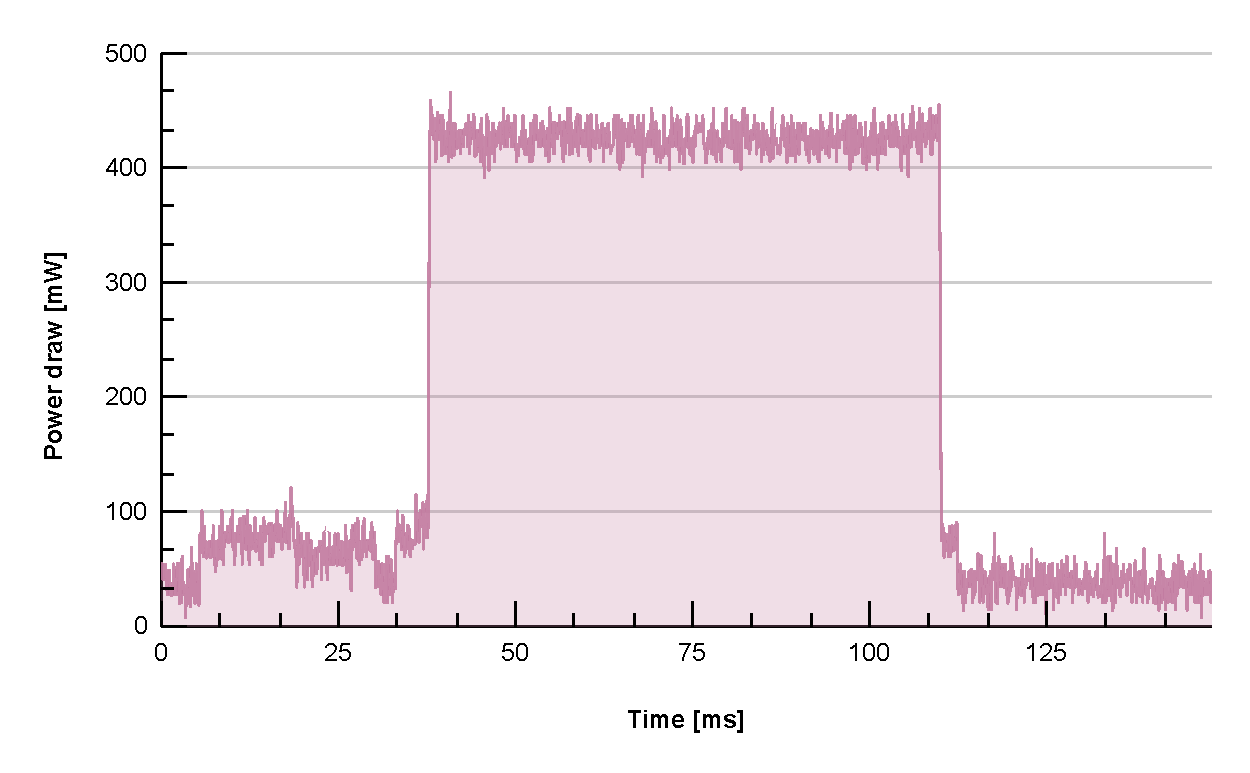
\includegraphics[width=1.0\textwidth]{images/lorawan_SF7_14dbm_125khz_power.pdf}
    \caption{Power draw during transmission of a LoRaWAN packet with payload size of 15 bytes, using SF7, 14dBm, 125kHz bandwidth}
    \label{LoRaWAN SF7}
\end{figure}
delta time is 71.8ms and total energy is 30.8mJ
